\documentclass{article}
\usepackage[utf8]{inputenc}
\usepackage{fancyhdr}
\usepackage{lastpage}
\usepackage{amsfonts}
\usepackage{amsmath}
\usepackage{amssymb}
\usepackage{bm}
\usepackage{graphicx}
\usepackage[shortlabels]{enumitem}
\usepackage[noabbrev, capitalise]{cleveref}

\usepackage{geometry}
 \geometry{
 a4paper,
 top=20mm,
 bottom=25mm,
 left=25mm,
 right=25mm,
 }



% define your IDs here:
\newcommand{\firststudentid}{305002206}
\newcommand{\secondstudentid}{313547911}

\pagestyle{fancy}
\fancyhf{}
\rhead{Written Solution for Assignment 1}
\chead{\firststudentid \qquad \secondstudentid}
\lhead{Natural Language Processing}
\rfoot{Page \thepage \hspace{1pt} of \pageref{LastPage}}
\renewcommand{\footrulewidth}{1pt}
 
\setlength{\parindent}{0pt}
\setlength{\parskip}{1em}
\renewcommand{\baselinestretch}{1.25}

\renewcommand{\thesubsection}{\thesection.\alph{subsection}}
\renewcommand{\thesubsubsection}{\thesubsection.\roman{subsubsection}}

\begin{document}

\refstepcounter{section}

\section{Understanding word2vec}
\subsection{}
assume $ x \in R^d$ and let $\vec{c}\in d$ be a vector with constant entries. 
\[
softmax(\vec{x} + \vec{c})_i =
\frac{\exp{(x_i+c)}}{\sum_{j=1}^{d}\exp{(x_j+c)}} =
\frac{\exp{x_i}\exp{c}}{\exp(c)\sum_{j=1}^{d}\exp{(x_j)}} =
\frac{\exp{x_i}}{\sum_{j=1}^{d}\exp{(x_j)}} =
softmax(\vec{x})
\]

\subsection{}
let y be one-hot vector.
\[
-\sum_{w \in W}y_w\log(\hat{y_w}) = 
-\sum_{w \neq o} 0*\log(\hat{y_w}) + (-\log(\hat{y_o})) =
log(\hat{y_o})
\]

\subsection{}
\[
J(\vec{V}_c, o, U) =
 -log(\frac {\exp(\vec{\mu_o^T}\vec{V_c})} {\sum_{w \in W}\exp(\vec{\mu_w^T}\vec{V_c}}) =
 log({\sum_{w \in W}\exp(\vec{\mu_w^T}\vec{V_c})} -  \vec{\mu_o^T}\vec{V_c}
\]
\[
\nabla_{\vec{v_c}(J)} = -\mu_o + \frac {1} {\sum_{w \in W}\exp(\vec{\mu_w^T}\vec{V_c})}  \sum_{r \in W}\vec{\mu_r}\exp(\vec{\mu_r^T}\vec{V_c}) = 
 \sum_{r \in W} \vec{\mu_r} \frac {\exp(\vec{\mu_r^T}\vec{V_c})} {\sum_{w \in W}\exp(\vec{\mu_w^T}\vec{V_c})} = 
\]
\[
 \sum_{r \in W} P(o=r) | C=c) \vec{\mu_r} - \vec{\mu_o} =
 \sum_{r \in W} (\hat{\vec y_r})\vec\mu_r - \vec\mu_0 = 
\]
\[
E[\vec\mu]_{\vec\mu \sim P(O|C=c)}-\vec\mu_0
\]

\subsection{}
for $w=0$:
\[
\nabla_{\vec\mu_w} = \vec V_c\exp(\vec\mu_w^T\vec V_c) \frac {1} {\sum_{r \in W}\exp(\vec{\mu_r^T}\vec{V_c})} - \vec V_c =
\vec V_c [(\hat{\vec Y_w}) - 1]
\]
for $w\neq 0$:
\[
\nabla_{\vec\mu_w} = \vec V_c (\hat{\vec Y})_w
\]
\subsection{}
since 6 is applied element-wise, the entries of the derivative vector will be the derivative of $\sigma x_i$ w.r.t for each entry i.
thus, will calculate the derivative for single element $x_i$:
\[
\frac {\partial\sigma(x_i)}{\partial x_i} = -\frac {1} {(1+\exp(-x_i))^2} (-\exp^{-x_i}) =  -\frac {1+(-\exp^{-x_i})} {(1+\exp(-x_i))^2} -\frac {-1} {(1+\exp(-x_i))^2}  = 
\]
\[
\sigma(x_i)-\sigma^2(x_i) = \sigma(x_i)(1-\sigma(x_i)) = \sigma(x_i)  \sigma(-x_i) 
\]

\subsection{}

\[
\nabla_{\vec\mu_o}[J_{neg}] = 
-[\frac{1}{\sigma(\vec\mu_o^T V_c)} \sigma(\vec\mu_o^T V_c) \sigma(-\vec\mu_o^T V_c) V_c] - [\sum_{k=1}^{K} \frac{1}{\sigma(\vec\mu_k^T V_c)} \sigma(\vec\mu_k^T V_c) \sigma(-\vec\mu_k^T V_c) \vec O_{o \notin (\mu_1,..,\mu)}  = 
\]
\[
 = -\sigma(-\vec\mu_o^T V_c) V_c
\]

for $j\in(1,2...K)$:
\[
\nabla_{\vec\mu_j}[J_{neg}] = 
-[\frac{1}{\sigma(\vec\mu_o^T V_c)} \sigma(\vec\mu_o^T V_c) \sigma(-\vec\mu_o^T V_c) \vec O] - [\sum_{k=1}^{K} \frac{1}{\sigma(\vec\mu_k^T V_c)} \sigma(\vec\mu_k^T V_c) \sigma(-\vec\mu_k^T V_c) frac{\partial [-\mu_k^T\vec V_c]}{\partial \vec\mu_j})  = 
\]
\[
 = +\sigma(-\vec\mu_j^T V_c) V_c
\]

\[
\nabla_{\vec V_c}[J_{neg}] = 
-[\frac{1}{\sigma(\vec\mu_o^T V_c)} \sigma(\vec\mu_o^T V_c) \sigma(-\vec\mu_o^T V_c) V_c] - [\sum_{k=1}^{K} \frac{1}{\sigma(\vec\mu_k^T V_c)} \sigma(\vec\mu_k^T V_c) \sigma(-\vec\mu_k^T V_c) \vec\mu_k  =
\]
\[
\sum_{k=1}^{K} \sigma(\vec\mu_k^T\vec V_c) \vec\mu_k - \sigma(\vec\mu_o^T\vec V_c) \vec\mu_o 
\]

In naïve soft-max one has to update the parameters - going through the entire corpus in each iteration, whereas here, we only consider k "additional" vecotrs.

\refstepcounter{subsection}
\subsubsection{}
\[
\frac {\partial J_skip-gram}{\partial U} = \sum_{-M <= j <= M ; j \neq o } \frac {\partial (\vec V_c, W_{t+j}, U} {\partial U}
\]
\subsubsection{}
\[
\frac {\partial J_skip-gram}{\partial \vec V_c} = \sum_{-M <= j <= M ; j \neq o } \frac {\partial (\vec V_c, W_{t+j}, U} {\partial \vec V_c}
\]
\subsubsection{}
\[
\frac {\partial J_skip-gram}{\partial \vec V_w} = 0
\]

\newpage

\section{Implementing word2vec}
\setcounter{subsection}{4}
\subsection{}

\begin{figure}
  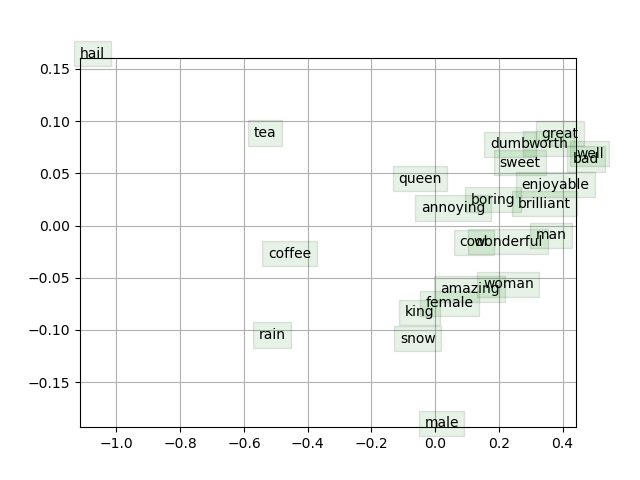
\includegraphics[width=\linewidth]{word_vectors.png}
  \caption{Word Vetors  SVD plot}
  \label{word_vectors}
\end{figure}

In figure \ref{word_vectors} we can see several intersting phenomena, regarding the clusters, trends and algebric operations.
\subsubsection{clusters}
The most disticnt cluster, appears on the top right corner of the plot. It includes words such as ("great", "sweet", "dumb") and others, all can be seen in figure \ref{word_vectors}. all words in this cluster are adjectives.
when looking at the left cluster, which is less distinctive, since words are further away from each other, we can see nouns (tea, coffee, rain, hail). The reasons why these words are not clustered as well could be several: their appearnces on the text might be too little, or biased (women drink tea, men drink coffee), or the sub dimension we are looking at ommits their relationship. 
In the middle, we can see a sub-cluster when looking at x values - king, queen, male, female. These words are considered as nouns, but they somewhat describe an object (king as a title for a man). We might be enforcing here what we wish to see, but it makes sense in the (x,y) coordinate system and according to the word2vec article.

\subsubsection{trends}
When looking at x-axis trends, we see the change from nouns (hail, tea, coffee) to adjectives (great, well, bad). In the middle we see titles (king, queen, etc.). For some reason, the word snow appears closer to king and female, than to rain. This of course doesn't support our conclusions, but we suspect it to be an outlier, brought-forth by biased text or the specific dim-reduction applied in SVD.
On the y-axis, we couldn't see any clear trends.
\subsubsection{algebric operations}
Like word2vec suggested, we tried to perform some algerbric operations. Below is an evaluation of word-coordinates using the grid we added to the plot.
lets take a look at the words:

\[king: (x = -0.10, y = -0.09)\]
\[male: (x = -0.03, y = -0.19)\]
\[female: (x = -0.03, y = -0.08)\]
\[queen: (x = -0.12, y = 0.04)\]
\[result = king - male + female = (-0.1, 0.02)\]

when using $L_2$ as distance function, annoted d, \[d(result, queen)=0.02\] thus makes it the closest vector to results. 


\end{document}